\chapter{Architecture logicielle}

\begin{figure}
	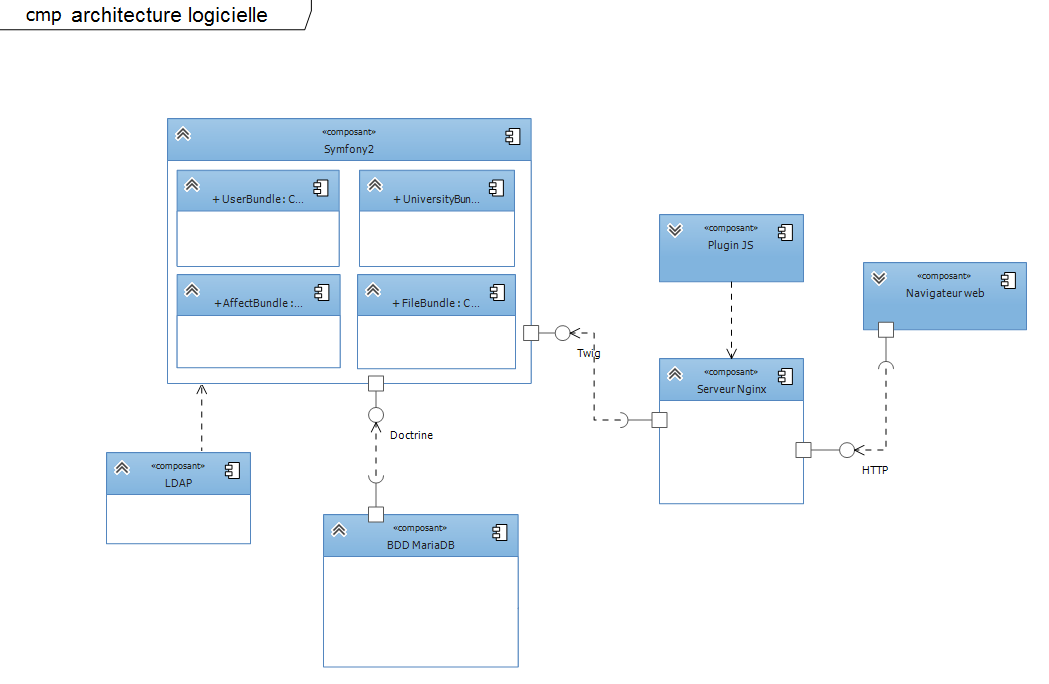
\includegraphics[scale=0.8,angle=90]{images/archilogi.png}
	\caption{Architecture des composants de l'application}
	\label{archilogi}
\end{figure}

La figure \ref{archilogi} présente l'organisation des différents modules de notre application. 
\bigbreak
Ayant utilisé le framework Symfony2, les différents modules sont séparés en bundles. Chaque bundle est un ensemble de fichiers permettant d'implémenter un groupe de fonctionnalités. Notre projet dispose de 4 bundles :
\begin{itemize}
	\item UserBundle qui gère les actions de l'utilisateur sur le site;
	\item UniversityBundle qui permet d'accéder à la liste d'université ou d'en modifier des entrées;
	\item AffectBundle qui gère les vœux et affectations des étudiants.
	\item FileBundle qui gère les documents administratifs déposés sur le site.
\end{itemize}
Chacun d'entre eux sera développé plus en détails dans les chapitres suivants.
\bigbreak

Même si le projet Symfony2 forme le corps de l'application,  d'autres modules sont indispensables au fonctionnement :
 
\section{Base de données}

L'architecture de la base de donnée sera décrite plus en détail dans le chapitre 7. 
Nous utilisons MariaDB, gestionnaire libre de base de données.
\bigbreak
Doctrine est un bundle inclut dans Symfony2, c'est un ORM (Object-Relational Mapping) que nous utilisons pour accéder à la base de données. Il permet principalement d'adresser des requêtes dans les codes PHP.

\section{Hébergement}

L'application est hébergée sur un serveur Nginx qui fait le lien entre la base de données et l'application Symfony2. Le serveur est lui-même hébergé au CRI et possède une capacité de 30 Go. Le CRI a aussi mis à disposition les clés pour passer le site en https, garantissant une meilleure sécurité.

\section{LDAP}

L'application est en contact avec les LDAP (annuaire) de l'INSA de Rennes.
Les administrateurs peuvent charger les étudiants directement depuis le LDAP. Il est aussi lors de l'authentification : notre application vérifie d'abord la présence dans sa base de donnée, puis interroge le LDAP qui vérifie le mot de passe. Ces derniers ne sont jamais enregistrés par notre application. 